\documentclass[../report.tex]{subfiles}
\begin{document}	

\chapter{Design and simulation}
\gls{tpr} can be achieved in different ways, discussed in section \ref*{sec:active_pr}. In this thesis, the goal is to achieve \gls{tpr} using MEMS for a broadband spectrum including C and L bands. Moreover, the idea is to optimize the design to achieve high \gls{per} and low \gls{il}.  
	
	\section{Approach}
	\gls{tpr} with MEMS can be approached in 2 ways. In the first approach, an asymmetric structure can be introduced in a straight waveguide to break its symmetry and in the process the polarization of the optical wave is rotated after transmission through the waveguide. Then another MEMS tunable waveguide can be introduced which reintroduces symmetry in the effective waveguide and as a result impedes polarization rotation. In the second approach, the technique is reversed i.e. the MEMS tunable waveguide is used to introduce asymmetry in the effective waveguide structure which rotates polarization. Without the MEMS structure the polarization is not rotated. In the design principles of the \gls{tpr}, the first approach is being followed.  
	
	\section{Designing the experiment}
	To design the geometry of the waveguide standard mode solver softwares are used. Both, Comsol\cite{comsol_2015} and CST \cite{cst_2015} are used to solve the modes in equation \ref{eq:helmholtz_eq_wg_general}. Mostly, in this thesis Comsol is used to find and optimize the port modes in 2-D geometry. Whereas, CST is used to optimize the 3-D structure using the S-parameters obtained for various port modes after running the simulation. 
		
		\subsection{Design principle}
To design a \gls{pr} in quantum scale, precision is a key factor. Index profile of chosen Silicon can also affect the structural dimensions of the design in a rigorous manner. Meshing of the geometry, cladding dimensions and its material composition, frequency domain of the solvers etc. are the key things to watch for in designing the simulation in the mode solver softwares. As the idea is to make the \gls{tpr} as broadband as possible, it is necessary to frequency analysis simulation for a wide-band spectrum in which the optical fibers for telecommunications work. As, the operating wavelength of the telecommunications optical fiber network in C-band and L-band are between $\SI{1530}{\nano\metre}$ and $\SI{1625}{\nano\metre}$, the corresponding frequency domain becomes $\SI{184.48}{\THz}$ - $\SI{195.94}{\THz}$.

\begin{equation}\label{eq:wg_width_param}
Base_{width} = Rib_{width} + Slab_{width} 
\end{equation}
  
	
		\subsection{Design A: Single stair Si waveguide on SOI with air cladding}

\subsubsection{Optimized dimensions of bus waveguide}

\begin{figure}[H] %h
	\centering
	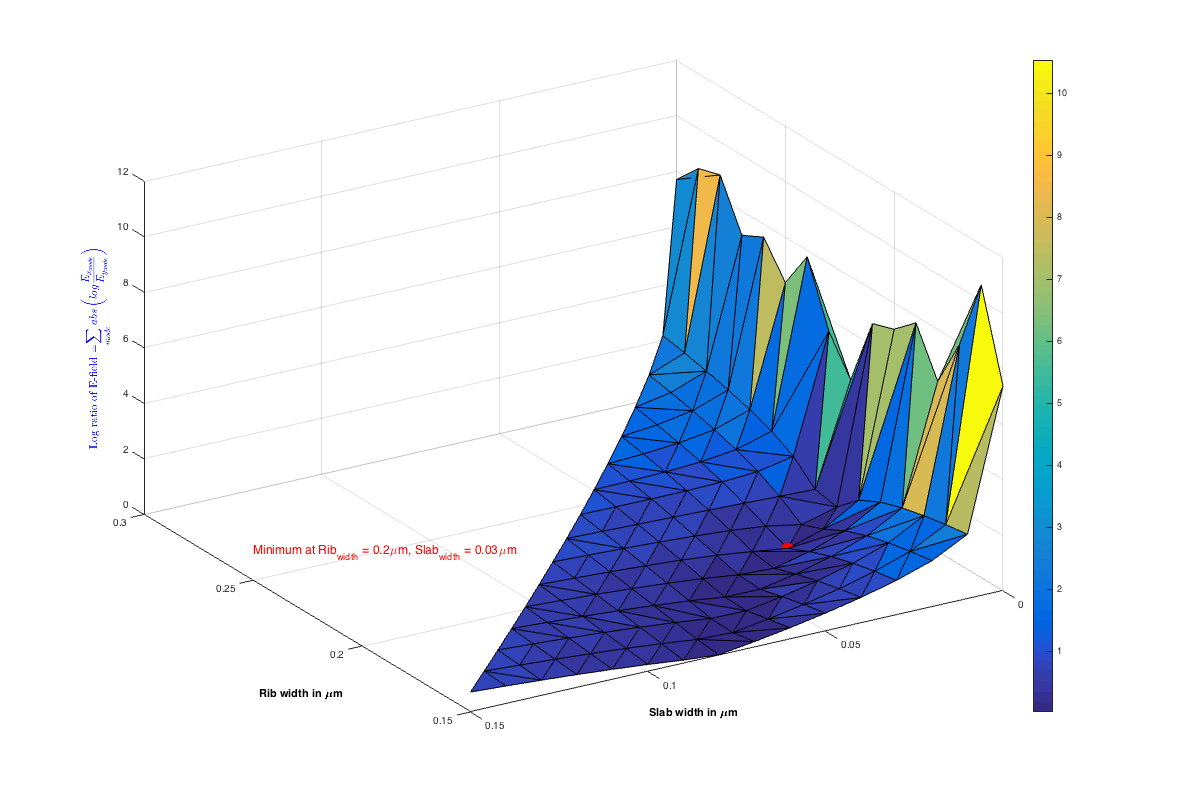
\includegraphics[width=1\textwidth]{3-graph-mode-sum}
	\caption{Summation of real part of absolute value of the logarithmic ratio of $E_x$ and $E_y$ fields plotted against rib and slab width in an area chart using MATLAB}
	\label{fig:3_graph_mode_sum}
\end{figure}

$\sum _{mode}Real\left| \log _{10}\dfrac {E_{X_{mode}}} {E_{Y_{mode}}}\right| \rightarrow 0$. Since, at $45{^\circ}$, $E_X \approx E_Y$. Hence, $\dfrac {E_{X_{mode}}} {E_{Y_{mode}}} \rightarrow 1$    

\begin{figure}[H] %h
	\begin{subfigure}[t]{0.45\textwidth}
		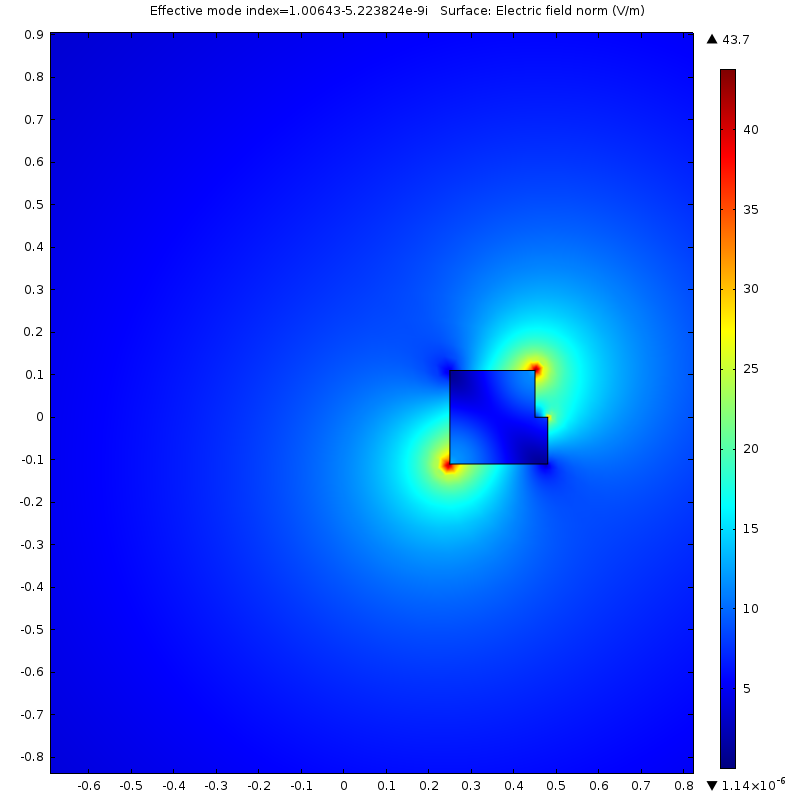
\includegraphics[width=\textwidth]{3-mode1-200-230}
		\caption{$1^{st}$ hybrid mode in the cross-section}
		\label{fig:3_mode1_200_230}
	\end{subfigure}
	\hfill
	\begin{subfigure}[t]{0.45\textwidth}
		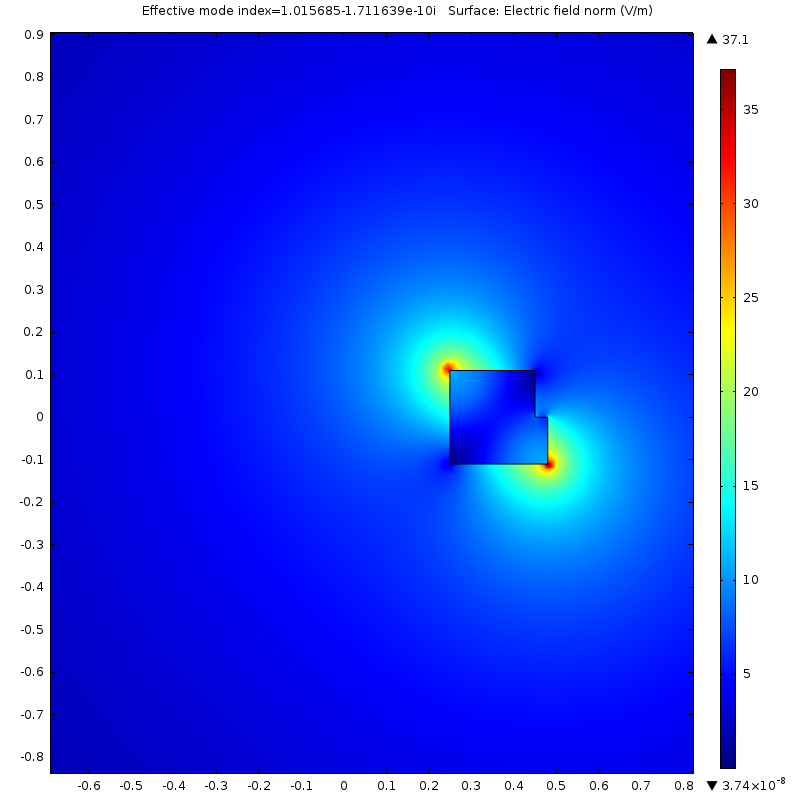
\includegraphics[width=\textwidth]{3-mode2-200-230}
		\caption{$2^{nd}$ hybrid mode in the cross-section}
		\label{fig:3_mode2_200_230}
	\end{subfigure}
	\caption{Hybrid modes in the cross-section with Rib width = 200nm, Rib height = 110nm, Slab width = 30nm, Slab height = 110nm, obtained using Comsol 2-D simulation}
\end{figure}

\begin{figure}[H] %h
	\begin{subfigure}[t]{0.45\textwidth}
		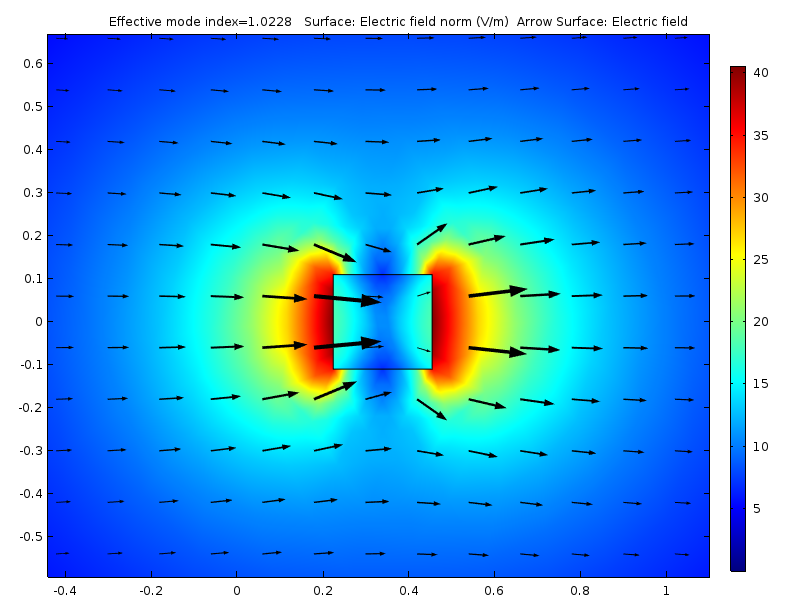
\includegraphics[width=\textwidth]{3-mode1-230-230}
		\caption{\gls{te} mode in the cross-section}
		\label{fig:3_mode1_230_230}
	\end{subfigure}
	\hfill
	\begin{subfigure}[t]{0.45\textwidth}
		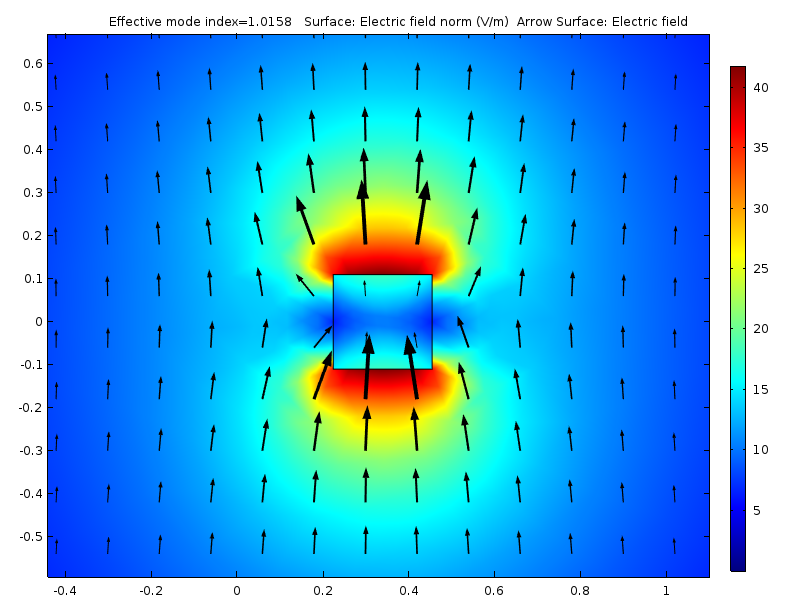
\includegraphics[width=\textwidth]{3-mode2-230-230}
		\caption{\gls{tm} mode in the cross-section}
		\label{fig:3_mode2_230_230}
	\end{subfigure}
	\caption{Hybrid modes in the cross-section with width = 230nm, height = 220nm, obtained using Comsol 2-D simulation}
\end{figure}

\begin{figure}[H] %h
	\centering
	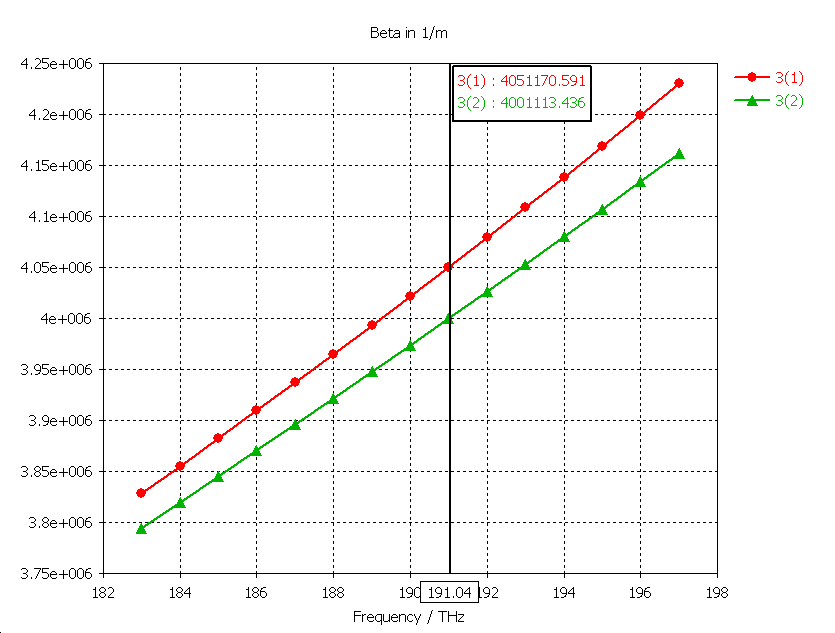
\includegraphics[width=0.9\textwidth]{3-effective-ri-200-230}
	\caption{Simulated effective \gls{ri} profile for the port modes in the cross-section of Rib width = 200nm, Rib height = 110nm, Slab width = 30nm, Slab height = 110nm, obtained using CST 3-D simulation}
	\label{fig:3_effective_ri_200_230}
\end{figure}


\begin{figure}[H] %h
	\centering
	\includegraphics[width=0.9\textwidth]{3-wg-design-1}
	\caption{Design of single-stair waveguide with initial dimensions at the port as width = 230nm and height = 220 nm. Stair cross-section dimensions are: Rib width = 200nm, Rib height = 110nm, Slab width = 30nm, Slab height = 110nm, and cross-section length = \SI{51}{\micro\meter}. The output port is along the Z-axis}
	\label{fig:3_wg_design_1}
\end{figure}

\begin{figure}[H] %h
	\centering
	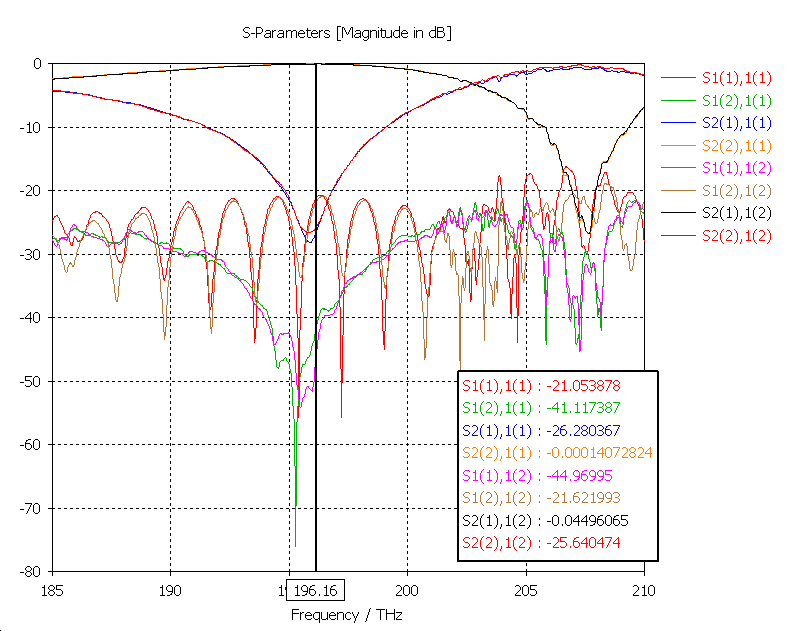
\includegraphics[width=0.9\textwidth]{3-stair-s-param-200-230}
	\caption{Simulated S-parameters in the single-stair waveguide with initial dimensions at the port as width = 230nm and height = 220 nm. Stair cross-section dimensions are: Rib width = 200nm, Rib height = 110nm, Slab width = 30nm, Slab height = 110nm, and cross-section length = \SI{51}{\micro\meter} obtained using CST 3-D simulation}
	\label{fig:3_stair_s_param_200_230}
\end{figure}

\subsubsection{Optimized dimensions of MEMS waveguide}
\begin{figure}[H] %h
	\centering
	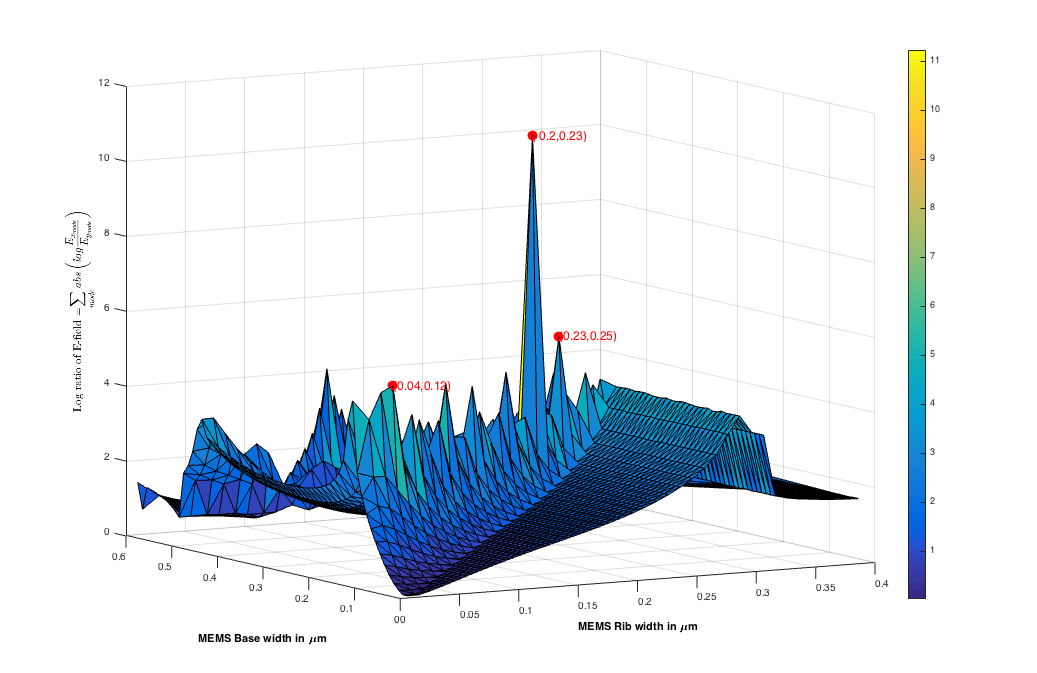
\includegraphics[width=1\textwidth]{3-graph-mode-sum-mems}
	\caption{Summation of real part of absolute value of the logarithmic ratio of $E_x$ and $E_y$ fields plotted against rib and total width in an area chart using MATLAB}
	\label{fig:3_graph_mode_sum_mems}
\end{figure}

$\sum _{mode}Real\left| \log _{10}\dfrac {E_{X_{mode}}} {E_{Y_{mode}}}\right| \rightarrow \infty$. Since, at TE or TM mode, $E_X \gg E_Y$, or $E_Y \gg E_X$. Hence, $\dfrac {E_{X_{mode}}} {E_{Y_{mode}}} \rightarrow \infty$ or $\dfrac {E_{Y_{mode}}} {E_{X_{mode}}} \rightarrow \infty$, depending on \gls{te} or \gls{tm}-mode.

		
\begin{figure}[H] %h
	\begin{subfigure}[t]{0.45\textwidth}
		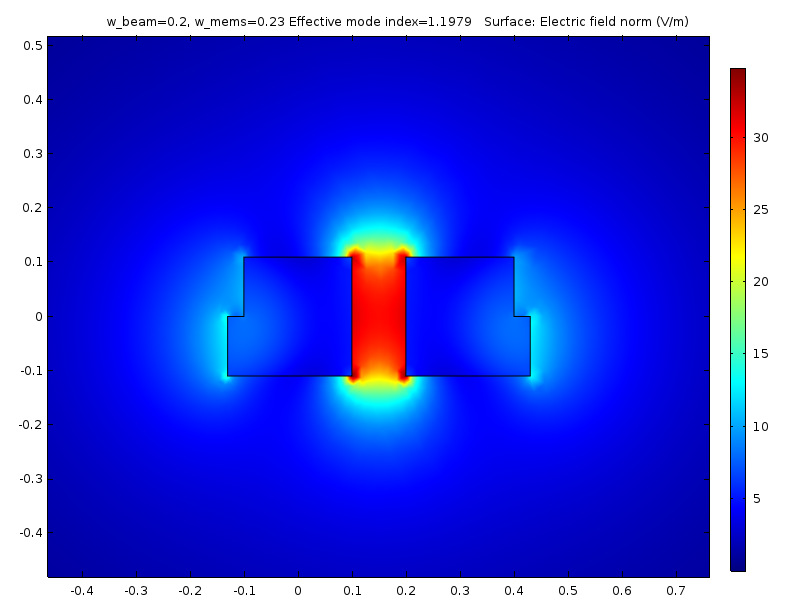
\includegraphics[width=\textwidth]{3-mems-mode1-200-230}
		\caption{\gls{te} mode with the \gls{mems} cross-section}
		\label{fig:3_mems_mode1_200_230}
	\end{subfigure}
	\hfill
	\begin{subfigure}[t]{0.45\textwidth}
		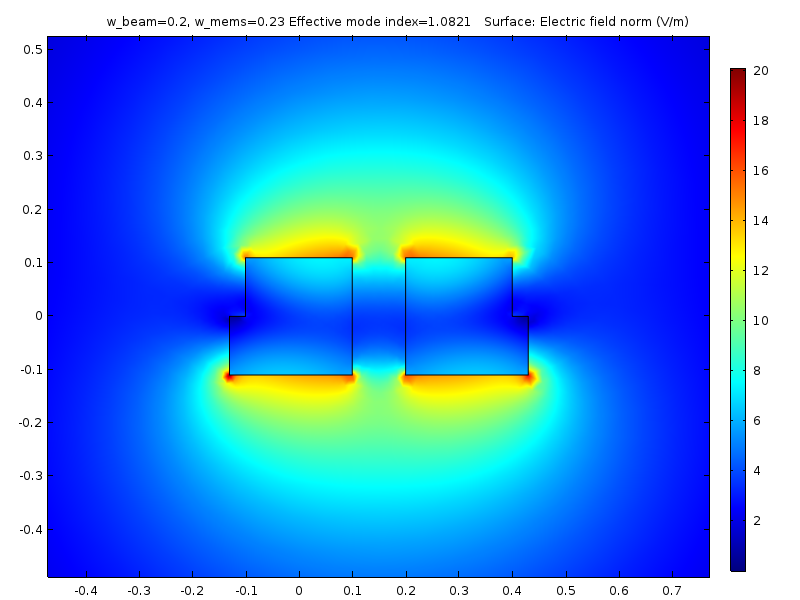
\includegraphics[width=\textwidth]{3-mems-mode2-200-230}
		\caption{\gls{tm} mode with the MEMS cross-section}
		\label{fig:3-mems-mode2-200-230}
	\end{subfigure}
	\caption{Modes in the cross-section with Rib width = 200nm, Slab width = 30nm, Slab height = Rib height = 110nm, in both bus and \gls{mems} waveguide, obtained using Comsol 2-D simulation}
\end{figure}


\subsubsection{Device tolerance}

\begin{figure}[H] %h
	\centering
	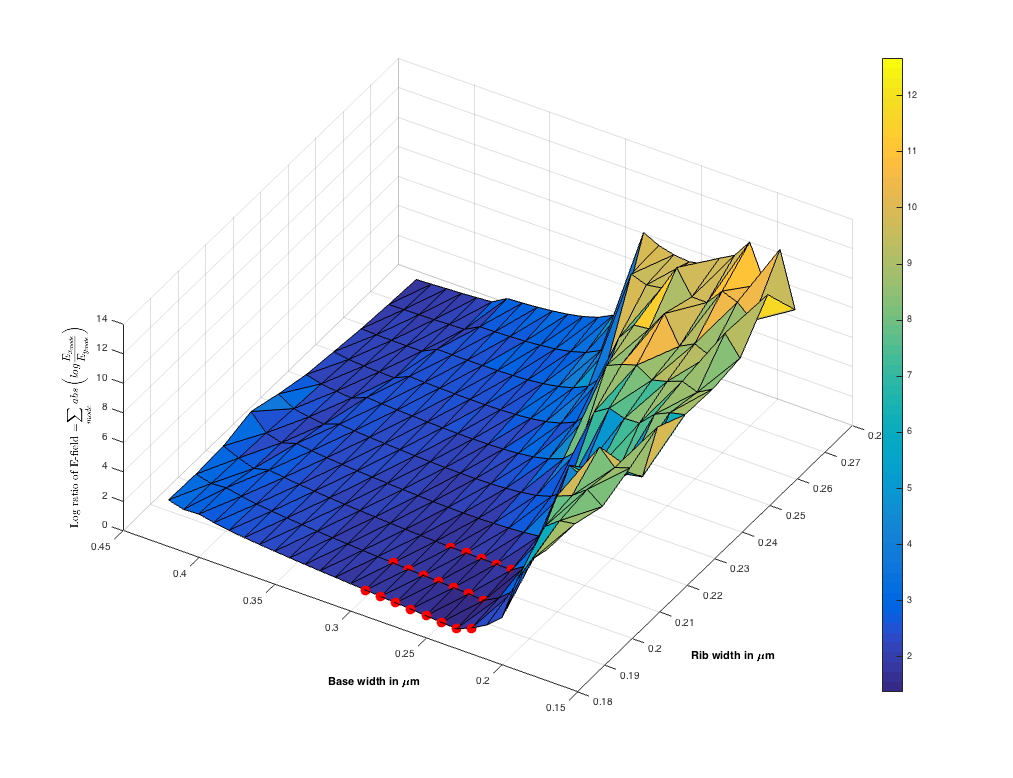
\includegraphics[width=1\textwidth]{3-graph-mode-sum-120nm-slab-height}
	\caption{20 least values, representing the summation of real part of absolute value of the logarithmic ratio of $E_x$ and $E_y$ fields, plotted against rib and total width in an area chart using MATLAB for Slab height = 120nm}
	\label{fig:3_graph_mode_sum_120nm_slab_height}
\end{figure}

\begin{figure}[H] %h
	\centering
	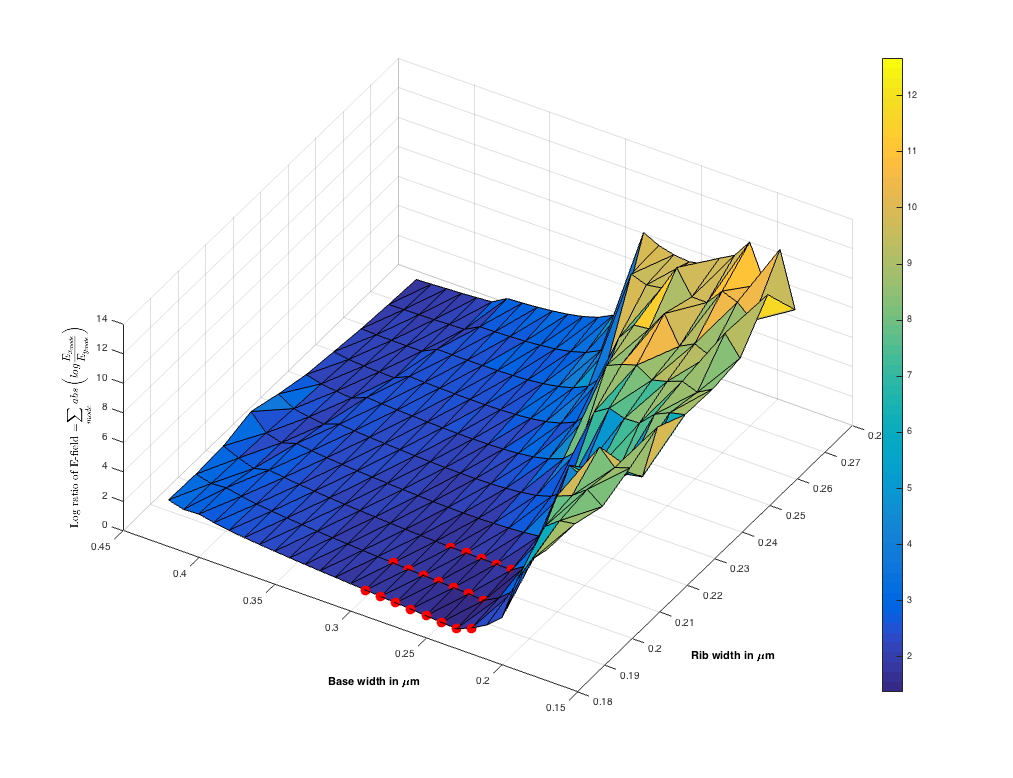
\includegraphics[width=1\textwidth]{3-graph-mode-sum-120nm-slab-height}
	\caption{20 least values, representing the summation of real part of absolute value of the logarithmic ratio of $E_x$ and $E_y$ fields, plotted against rib and total width in an area chart using MATLAB for Slab height = 90nm}
	\label{fig:3_graph_mode_sum_90nm_slab_height}
\end{figure}
				
		\subsection{Design B: Tapered Si waveguide with horizontal gradual asymmetry on SOI with air cladding}
		
\begin{figure}[H] %h
	\begin{subfigure}[t]{0.45\textwidth}
		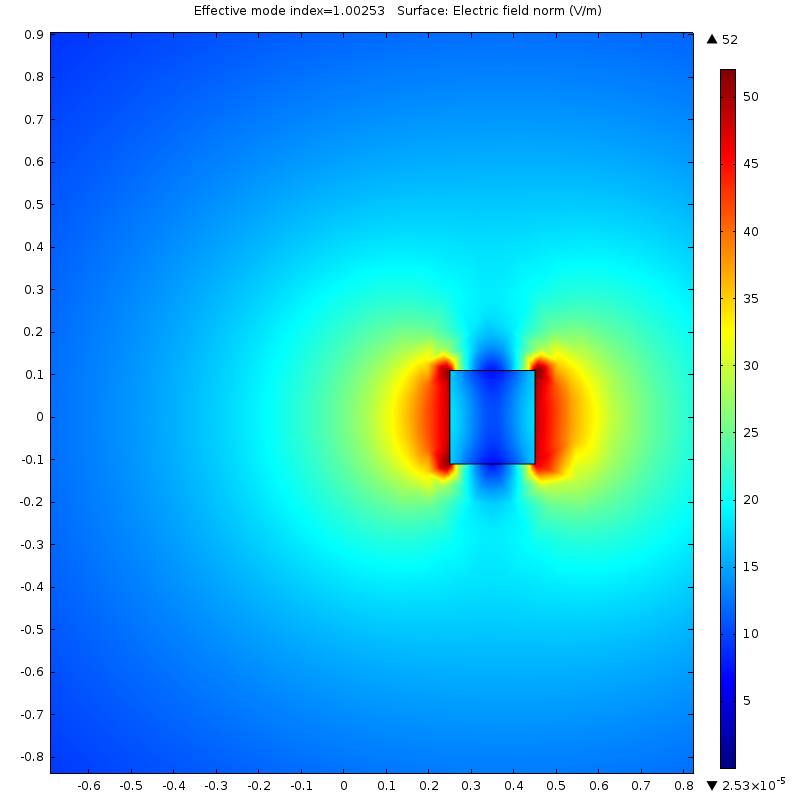
\includegraphics[width=\textwidth]{3-mode1-200-200}
		\caption{\gls{te} mode in the cross-section}
		\label{fig:3_mode1_200_200}
	\end{subfigure}
	\hfill
	\begin{subfigure}[t]{0.45\textwidth}
		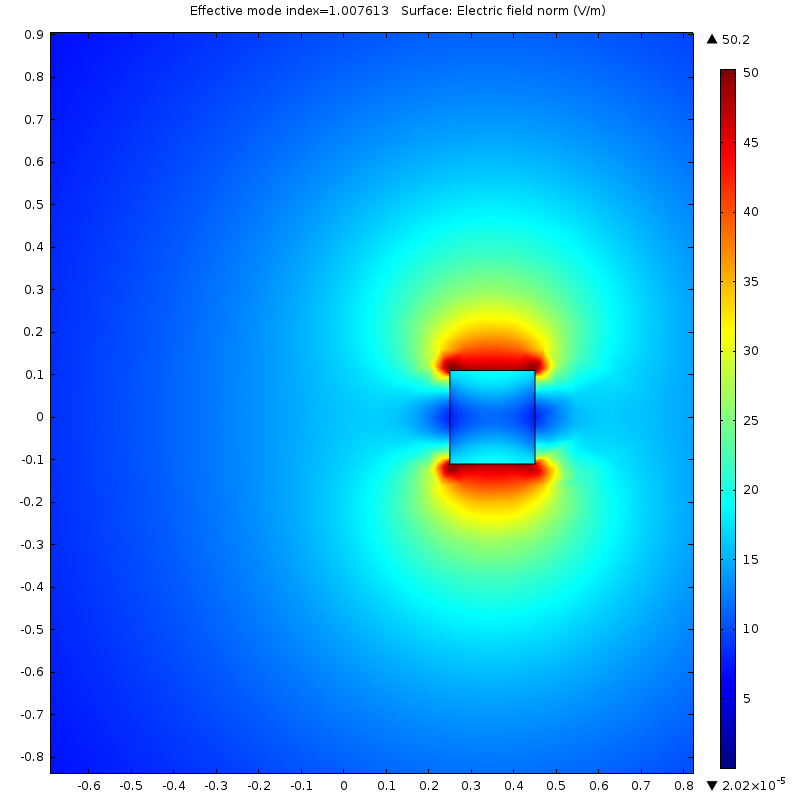
\includegraphics[width=\textwidth]{3-mode2-200-200}
		\caption{\gls{tm} mode in the cross-section}
		\label{fig:3_mode2_200_200}
	\end{subfigure}
	\caption{Hybrid modes in the cross-section with width = 200nm, height = 220nm, obtained using Comsol 2-D simulation}
\end{figure}
	
	\section{Simulation results and analysis}
	
\end{document}
